\documentclass[11pt]{article}
\usepackage{graphicx}
\usepackage{caption}
\usepackage{subcaption}
\usepackage[section]{placeins}
\usepackage{float}
\usepackage{amsmath}
\usepackage{mathtools}
\usepackage{changepage}  
\usepackage{apacite}

\bibliographystyle{apacite}
\setlength{\columnsep}{1cm}

\newlength{\offsetpage}
\setlength{\offsetpage}{1.5cm}
\newenvironment{widepage}{\begin{adjustwidth}{-\offsetpage}{-\offsetpage}%
    \addtolength{\textwidth}{2\offsetpage}}%
{\end{adjustwidth}}


\newcommand{\triplefigure}[3]{
\begin{figure}[H]
  \centering
  \begin{minipage}{0.3\textwidth}
    \centering
    \includegraphics[width=\textwidth]{#1}
  \end{minipage}
  \begin{minipage}{0.3\textwidth}
    \centering
    \includegraphics[width=\textwidth]{#2}
  \end{minipage}
  \begin{minipage}{0.3\textwidth}
    \centering
    \includegraphics[width=\textwidth]{#3}
  \end{minipage}
\end{figure}
}
\newcommand{\doublefigure}[2]{
\begin{figure}[H]
  \centering
  \begin{minipage}{0.45\textwidth}
    \centering
    \includegraphics[width=\textwidth]{#1}
  \end{minipage}
  \begin{minipage}{0.45\textwidth}
    \centering
    \includegraphics[width=\textwidth]{#2}
  \end{minipage}
\end{figure}
}
\newcommand{\singlefigure}[1]{
\begin{figure}[H]
  \centering
  \begin{minipage}{0.4\textwidth}
    \centering
    \includegraphics[width=\textwidth]{#1}
  \end{minipage}
\end{figure}
}
\newcommand{\singlewiderfigure}[1]{
\begin{figure}[H]
  \centering
  \begin{minipage}{0.65\textwidth}
    \centering
    \includegraphics[width=\textwidth]{#1}
  \end{minipage}
\end{figure}
}

\let\oldabs\abs % Store original \abs as \oldabs
\let\abs\undefined % "Undefine" \abs
\DeclarePairedDelimiter\abs{\lvert}{\rvert}

\begin{document}
\begin{titlepage}
  \centering
  \vfill
  \vfill
  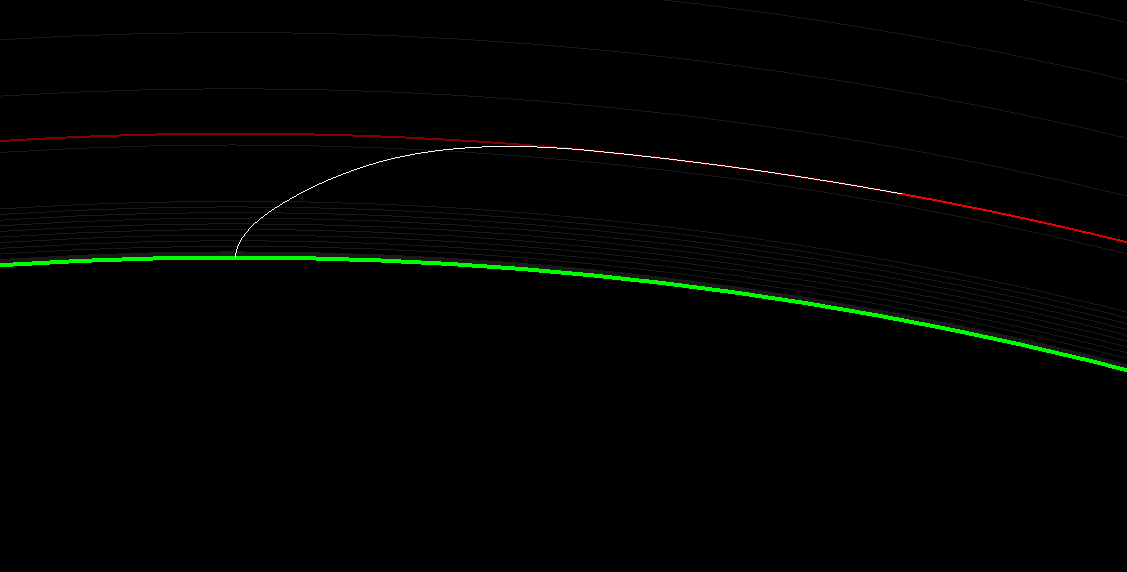
\includegraphics[width=0.5\textwidth]{./220km.png}
  \vskip3cm
  {\Large
  \textbf{Optimizing the ascent trajectory for an orbital class launch vehicle}\\
  \vskip0.25cm
  Final project in SI1336\\
      \vskip1cm
      Erik Weilow\\
      \vskip0.5cm
      \today\\
  }    
  \vfill
  \vfill
\end{titlepage}
\newpage

\section{Introduction}
The goal of this project is to compare the fuel consumption for the launch of a multi-stage orbital class launch vehicle into low Earth orbit, from an equatorial and a polar launch site.
To do this, the project formulates an approximate model of the conditions encountered for the launch vehicle during ascent as well as a simple control algorithm.
To be able to draw conclusions from the results gained, the control algorithm must be optimized. 
This will be done using a randomized optimization algorithm.
The project is thus split into four major parts: the equations describing the state of the rocket, the physics model, the ascent guidance algorithm as well as the optimization of control parameters.

\section{Equations of the rocket}
A rocket works on the principle of momentum conservation. Mass is ejected at a rate $\dot{m}$ (mass flow) through the engines at a velocity $v_{e} = I_{sp} / g_{_0}$, 
producing a thrust $F = \dot{m} \cdot v_{e} = \dot{m} \cdot I_{sp} / g_{_0}$. If we can calculate these parameters at all times, we can simulate a rocket.

To complicate things further, we need to consider that the rocket has several stages.
This can be solved by letting the state of the rocket be described with position, velocity and \textit{expended mass} ($m_e$):
$$
S = (\vec{r}, \vec{v}, m) = (x, y, z, v_x, v_y, v_z, m_e)
$$
where $m_e$ is the integral of exhaust mass flow (ejected mass) over time:
$$
m_e(t) = \int_0^t \dot{m}(S,t) dt
$$

The reason for including expended mass in the model is that it lets us derive the currently active stage, 
as well as the necessary variables (thrust, mass and mass flow) of the rocket as a function of used propellant. 

\subsection{Input parameters}
Consider each stage of the rocket as collection of parameters:
\begin{center}
\begin{tabular}{ r  | l  }
  Parameter & Description \\
  \hline
  $m_{prop,i}$ & Propellant mass of stage \\
  $m_{dry,i}$ & Dry mass of stage (without propellant) \\
  $F_{sl,i}$ & Thrust at sea level pressure \\
  $F_{vac,i}$ & Thrust in vacuum pressure \\
  $I_{sp,sl,i}$ & Specific impulse at sea level \\
  $I_{sp,vac,i}$ & Specific impulse in vacuum pressure
\end{tabular}
\end{center}

such that each stage $i=0,1,2...$ can be written
$$
s_i = (m_{prop,i}, m_{dry,i}, F_{sl,i}, F_{vac,i}, I_{sp,sl,i}, I_{sp,vac,i})
$$

Furthermore, a rocket typically has an aerodynamic shell (fairing) that is deployed around the edge of space (100km). This is modelled simply by the parameters
\begin{center}
  \begin{tabular}{ r  | l  }
    Parameter & Description \\
    \hline
    $m_i$ & Mass of fairing \\
    $h_{deployment,i}$ & Altitude of deployment
  \end{tabular}
\end{center}
such that each fairing $i=0,1,2...$ can be written
$$
f_i = (m_i, h_{deployment,i})
$$

Lastly, the payload of the rocket is modelled as a mass $m_{payload}$.

\subsection{Derived parameters}
To run simulations of defined by the parameters in the previous section, 
we need to derive the current mass of the entire rocket. This is not as simple as subtracting $m_e$ from the initial mass, as we want to model staging.
Instead consider parameters driven by the currently active stage $s_{active}$.

\subsubsection{Mass}

If the propellant of stages before $s_i$ is
$$
m'_{prop,i} = \sum_{j=0}^{i-1} m_{prop,j}
$$
then the currently active stage fulfill the criteria
$$
m'_{prop,active} < m_e(t) < m'_{prop,active} + m_{prop,active}
$$

As we are only considering a two stage launch vehicle, the active stage can be defined by
$$
s_{active} = \begin{cases} 
  s_0 & : m_e < m_{prop,0} \\
  s_1 & : 0 < m_e - m_{prop,0} < m_{prop,1}
\end{cases}
$$

If the mass of stages after the stage $s_i$ is
$$
m'_{stages,i} = \sum_{j=i+1} m_{prop,j} + m_{dry,j}
$$
This defines the current mass of stages, when $s_{i}$ is active, as
$$
m_{stagemass,i} = \left( m_e(t) - m'_{prop,i} \right) + m_{dry,i} + m'_{stages,i}
$$

If $h_{max}$ is the maximum altitude reached up until time $t$, then the mass of fairings currently on the rocket can be described by the sum
$$
m_{fairings}(h_{max}) = \sum_{i=0} m_i (1 - H(h_{max} - h_{deployment,i}))
$$

Thus, the total instantaneous mass for an active stage $s_i$ is
$$
m_i = m_{stagemass,i} + m_{fairings}(h_{max}) + m_{payload}
$$

\subsubsection{Thrust}

Since the thrust of a rocket propulsion system is linear in the pressure difference between the exhaust and surrounding pressure, 
it is assumed in our model that the thrust $F$ changes linearly between $F_{sea}$ and $F_{vacuum}$ with pressure $p$~\cite{thrust}.
%
% https://www.grc.nasa.gov/www/k-12/rocket/thrsteq.html
%

For a given active stage $s_i$, if pressure is written as a function of altitude $h$, thrust can be written as 
$$
F_i(p(h)) = F_{sl,i} + \left( F_{sl,i} - F_{vac,i} \right) \frac{p(h)}{p(0)}
$$

This only holds if the stage has remaining fuel ($m_e - m_{prop,i} > 0$) 
otherwise 
$$
F_i(p(h)) = 0
$$

\subsubsection{Mass flow}
% 
% https://www.grc.nasa.gov/www/k-12/airplane/specimp.html 
%
Mass flow is necessary to find $m_e(t)$, and is given in a general form by \cite{massflow}:
$$
\dot{m} = \frac{F}{ g_0 I_{sp}}
$$

If we assume mass flow to be constant through the propulsion system, then $I_{sp}$ must share the same linear behaviour in pressure as thrust does.
Thus, for an active stage $s_i$, let
$$
I_{sp,i}(p(h)) = I_{sp,sl,i} + \left( I_{sp,sl,i} - I_{sp,vac,i} \right) \frac{p(h)}{p(0)}
$$

This gives the mass flow
$$
\dot{m}_i(p(h)) = \frac{F_i(p(h))}{ g_0 I_{sp,i}(p(h))}
$$

\subsubsection{Summarization}
To tie the equations together, we define the functions
$$
m(m_e) = m_i, \quad 
F(m_e, p(h)) = F_i(p(h)), \quad 
\dot{m}(m_e, p(h)) = \dot{m}_i(p(h)) \quad 
$$
where the active stage $s_i$ is derived from a given $m_e$.

\section{Physics model}
To simulate the ascent of the rocket, a model of the physics involved is required.

\subsection{Coordinate system}
The simulation uses two coordinate systems, one cartesian and one kinematic.
The cartesian system $\hat{x}, \hat{y}, \hat{z}$ is originated in the starting location and oriented such that
$\hat{x}$ points towards the wanted direction of orbit,
$\hat{y}$ points radially up, and $\hat{z} = \hat{x} \times \hat{y}$.

The kinematic system $\hat{r}, \hat{t}, \hat{z}$ follows the rocket and is oriented such that 
$\hat{r}$ is the normalized radial vector, $\hat{z}$ is the same as in the cartesian system, 
and the tangential vector is $\hat{t} = \hat{r} \times \hat{z}$. In a circular orbit, $\hat{t}$ is parallel to velocity $\vec{v}$.

\begin{figure}[H]
  \centering
  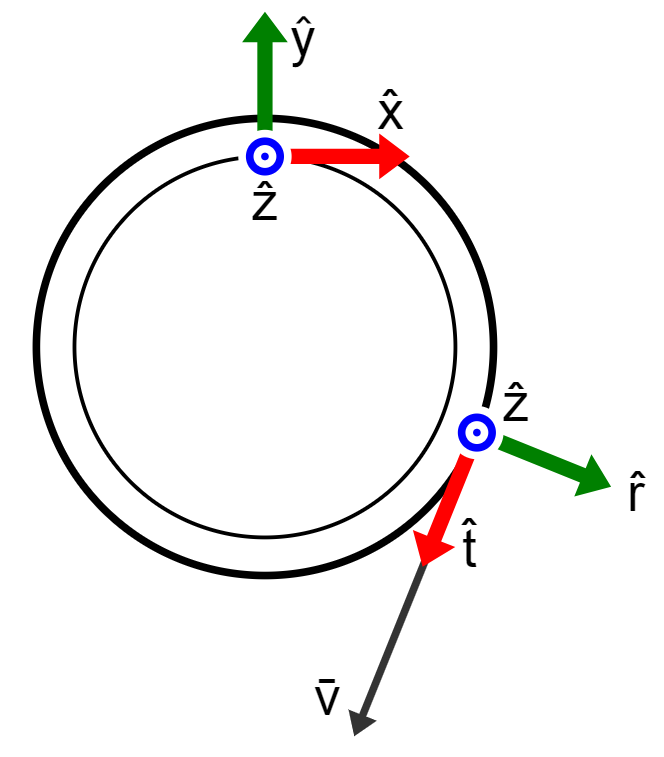
\includegraphics[width=0.45\textwidth]{./orbit.png}
  \caption{The instantaneous coordinates}
\end{figure}

\subsection{Atmosphere}
The atmosphere in the simulation is modelled according to the U.S Standard Atmosphere~\cite{atmosphere2014}.
%
% Here we write a bit about the american standard atmosphere model
%
Produces $\rho(r)$

\subsection{Forces}
In this model, it assumed that three forces are acting on the rocket: thrust $T$, aerodynamic drag $D$ and gravity $G$.

\subsubsection{Gravity - G}
Gravity is modelled based on the Newtonian formulation, resulting in a force
$$
\vec{G}(\vec{r}, m_e) = -m(m_e) \frac{\mu}{r^2} \hat{r} 
$$
where r is the distance to the center of Earth from the rocket, and $\mu \approx 3.986\cdot10^{14} m^3 s^{−2}$ is the standard gravitational parameter.

\subsubsection{Aerodynamic drag - D}
% 
% Include Drag equation
% Include atmospheric model incl. reference
% Include typical C_d
%
To model aerodynamic drag it first is assumed that the atmosphere, independently of radius, moves at a velocity:
$$
\vec{v}_{atm} (\vec{r}) = v_{surf} \cdot \hat{t}
$$
This allows the definition of the wind-relative velocity
$$
\vec{v}_{atm,rel} (\vec{r}, \vec{v}) = \vec{v} - \vec{v}_{atm} (\vec{r})
$$

%
% TYPICAL VALUE REFERENCE FROM OTHER PEOPLE THANKS
%
Under the assumption that the the drag equation holds for the entirety of the ascent, then
$$
\vec{D}(\vec{r}, \vec{v}, m_e) = - \frac{ m(m_e) \cdot  C_d  \cdot A \cdot \rho(r) }{2} {\left| \vec{v}_{atm,rel} (\vec{r}, \vec{v}) \right|}^2 \hat{v}
$$
% coefficient of drag $C_d = 0.2$, 
\subsubsection{Thrust - T}

%
% stuff about mass flow
%

To abstract the guidance algorithms from the physics model, it is assumed that guidance controls throttle as
$$
\eta = \eta(\vec{r}, \vec{v}, m_e, t)\in[0,1]
$$
and angle of thrust (AoT) from the vertical $\hat{r}$ as
$$
\theta = \theta(\vec{r}, \vec{v}, m_e, t)\in\left[0,\pi\right]
$$

Throttle and AoT interact such that 
$$
\vec{T}(\vec{r}, \vec{v}, m_e, t) = \left( \cos ( \theta ) \cdot\hat{r} + \sin ( \theta ) \cdot\hat{t} \right) \cdot F(m_e, P) \cdot \eta
$$

\subsection{Differential equation}
The combination of gravity, aerodynamic drag, and thrust give the equation
$$
\vec{a}(\vec{r}, \vec{v}, m_e) = \frac{1}{m_i} \left( G(\vec{r}, m_e) + D(\vec{r}, \vec{v}, m_e) + T(\vec{r}, \vec{v}, m_e, t) \right)
$$

\section{Ascent guidance}
The ascent guidance implemented in the simulation can be categorized into five phases:
\begin{itemize}
  \item Liftoff
  \item Kickpitch
  \item Gravity turn
  \item Orbital insertion
  \item Terminal guidance
\end{itemize}

\begin{figure}[H]
  \centering
  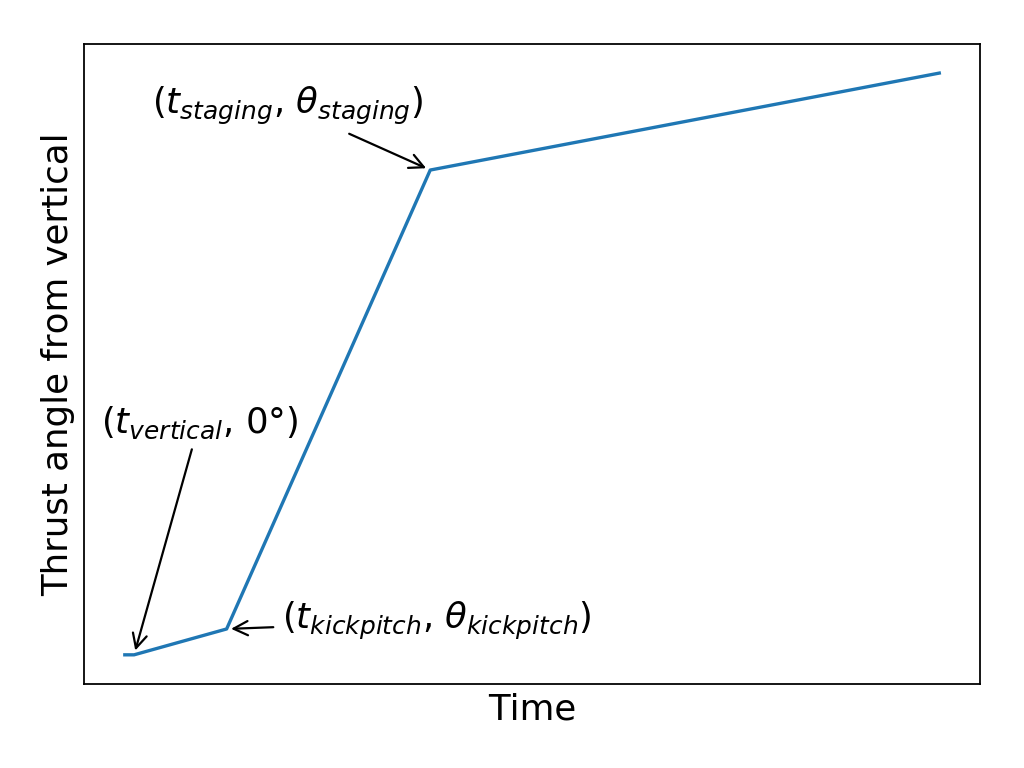
\includegraphics[width=0.8\textwidth]{./plots/angleFromVertical.png}
  \caption{Typical thrust angle from vertical (intentionally without units)}
\end{figure}

\subsection{Liftoff ($0 < t < t_{vertical}$)}
During this phase, the trajectory is entirely vertical - $\theta = 0$ and $\eta = 1$.

\subsection{Kickpitch ($t_{vertical} < t < t_{kickpitch}$)}
During this phase, the trajectory starts pitching towards the horizon slightly.
The angle $\theta$ is linearly interpolated between 0 and the defining parameter $\theta_{kickpitch} = 4^{\circ}$ according to
$$
\theta(t) = \theta_{kickpitch} \frac{t - t_{vertical}}{t_{kickpitch} - t_{vertical}}
$$

\subsection{Gravity turn ($\dot{m} t_{kickpitch} < m_e(t) < m_{prop,0}$)}
During the time between the end of kickpitch and the time of staging (when the expended mass is equal to the propellant in the first stage),
the angle $\theta$ is linearly interpolated between $\theta_{kickpitch}$ and the defining parameter $\theta_{staging}$ according to
$$
\theta(t) = \theta_{kickpitch} + \left( \theta_{staging} - \theta_{kickpitch} \right) \frac{m_e(t) - \dot{m} t_{kickpitch}}{m_{prop,0} - \dot{m} t_{kickpitch}}
$$

\subsection{Orbital insertion ($m_{prop,0} < m_e(t) < m_{prop,0} + m_{prop,1}$)}
This phase lasts until terminal guidance is triggered. The angle $\theta$ is interpolated from $\theta_{staging}$ to 0 according to
$$
\theta(t) = \theta_{staging} \left( 1 - \frac{m_e(t) - m_{prop,0}}{m_{prop,1}} \right)
$$

\subsection{Terminal guidance}
Terminal guidance is necessary to achieve a circular orbit within this simulation and previously mentioned ascent guidance parameters.
It consists of a PI-controller that attempts to cancel out any vertical velocity.

The conditions for entering terminal guidance is:
\begin{itemize}
  \item $h > g_{ap} - 55$
  \item OR:
  \item $h > 100$ and $\left| \vec{v} \cdot \hat{r} \right| < 50$
\end{itemize}

Within terminal guidance, $\theta$ is controlled with the regulator 
$$
\theta = 5 \cdot e(t) + 5 \int_{t_{triggered}}^t e(t') dt'
$$
where $t_{triggered}$ is the time at which terminal guidance was triggered, and
$$
e(t) = \vec{v} \cdot \hat{r}
$$

Furthermore, throttle is controlled by
$$
\eta = \begin{cases}
0 & : \quad r_{pe} > g_{pe} - 2 km, \quad g_{ap} - 2 km < r_{ap} < g_{ap} + 3 km \\
0 & : \quad r_{pe} > g_{pe} - 2 km, \left| \vec{v} \cdot \hat{r} \right| < 15 km \\
0.05 & : \quad r_{pe} > g_{pe} - 10 km \\
0.25 & : \quad r_{pe} > 0 km \\
0.5 & : \quad r_{pe} > -100 km \\
1 & :  \quad otherwise
\end{cases}
$$

If $\eta = 0$, the simulation ends in orbit.

\section{Integration}
The integration was done using a 4th order Runge-Kutta integrator on expended mass $m_e$, velocity $\vec{v}$ and position $\vec{r}$. 
This choice was made, because even though RK4 is not stable in terms of energy, it is simple to implement and produces low errors for the relatively short time spans simulated during a rocket launch (in the order of 500 seconds).
Relatively few large time steps are required to get a stable simulation, which is very useful when running an optimization algorithm, compared to other methods.

The choice of time step for the optimization step is detailed in the next section, but the final simulation is run in scaled real-time: such that we do $N$ steps per frame $\Delta t_f = 1/60 s$, resulting
in a time step of 
$$
\Delta t = 1/n \Delta  t_f = 1/(60N) s
$$ 
The simulation is then run as an animation with speed-up $n$, resulting in $n \cdot N$ time steps taken per frame. 
Going much higher, up to 10x more steps per frame, would be computationally possible but introduces
numerical inaccuracies. Being able to run the simulation in real-time means that it could also, in theory, be run on a real launch vehicle.

\subsection{Initial conditions}
For ease of simulation, the influence of launching from the equator is modelled as an initial horizontal velocity $v_{surf}$.
If the radius of Earth is denoted as $R_0$, then the initial conditions in the Cartesian frame are:
$$
\vec{r}_0 = R_0 \cdot \hat{y}, \quad \vec{v}_0 = v_{surf} \cdot \hat{x}, \quad m_e = 0
$$

Launch from the equator result in $v_{surf} \approx 440 m/s$ and launch from the poles result in $v_{surf} = 0 m/s$.

\section{Optimization of parameters}
To optimize parameters, an error function has to be established.
From introduction, we know that the goal is to reach a specific periapsis ($g_{pe}$) and apoapsis ($g_{ap}$). 
Let the periapsis from each simulation be $r_{pe}$, and the periapsis be $r_{ap}$.
As the terminal guidance algorithm works by eliminating vertical velocity, after reaching maximum altitude, we also want to make sure to use the maximum altitude reached ($h_{max}$).
To make sure the terminal guidance algorithm works well, we also want to use the altitude at which orbit is reached ($h$).
Since the project goal is to look at fuel usage for equatorial versus polar launch, it would be good to also use the fuel remaining after orbit insertion ($m_{final}$).

This lets us define the error function
$$
\begin{aligned}
E(r_{pe}, r_{ap}, g_{pe}, g_{ap}, h, h_{max}, m_{final}) = \\
\frac{{\left( r_{ap} - g_{ap} \right)}^2}{{\left( 10 \right)}^2} +
\frac{{\left( r_{pe} - g_{pe} \right)}^2}{{\left( 10 \right)}^2} +
\frac{{\left( h_{max} - g_{pe} \right)}^2}{{\left( 10 \right)}^2} +
\frac{{\left( h - g_{pe} \right)}^2}{{\left( 10 \right)}^2}
+ m_{final}
\end{aligned}
$$

This error function is used to score control algorithm parameters using a randomized optimization method, in which the ascent control parameters described below 
are randomly perturbated from the currently best choice of parameters using specific random radii and scaling, such that for each one: $parameter_{i+1} = parameter_{i} + scale \cdot \text{random}(-radii, radii)$
\begin{center}
  \begin{tabular}{ r | l  }
    Parameter & Random radius \\
    \hline
    $t_{vertical}$ & 1 \\
    $t_{kickpitch}$ & 4 \\
    $\theta_{staging}$ & 2 \\
    $a_{max}$ & 0.1 \\
  \end{tabular}
\end{center}

For every perturbation iteration $i$, a simulation is run at a specific timestep $\Delta t$ and iteration-specific scaling 
$ scale = s (5 - (i\,\text{mod}\,5)) / 5$.\footnote{This led to being able to converge faster} If the result is scored lower than the currently best score, the currently best choice of parameters are set to
the perturbated ones.
If the result is not scored lower, the perturbation is discarded.
This is done for different sets of time steps and scaling factors, progressively going to a finer time step, until either a max count of attempts have been reached or a minimum score is achieved according to the following sequence:
\begin{center}
  \begin{tabular}{ r | l | l | l  }
    Maximum score & Maximum runs & $\Delta t$ & Random scale ($s$) \\
    \hline
    10 & 10000 & 1 & 30 \\
    5 & 10000 & 1 & 15 \\
    5 & 10000 & 0.5 & 4 \\
    2 & 10000 & 0.5 & 2 \\
    1 & 10000 & 0.2 & 1 \\
    0.2 & 1000 & 0.1 & 1 \\
  \end{tabular}
\end{center}

The parameters that is considered best at the end of optimization is then used in a more accurate simulation to produce results.

\section{Results}
We'll start by looking at how well the guidance algorithm worked. Three goal orbits was optimized in the program, and we'll look at both how close it guided the rocket into the goal orbit as well as how much propellant was consumed.

\begin{figure}[H]
  \centering
  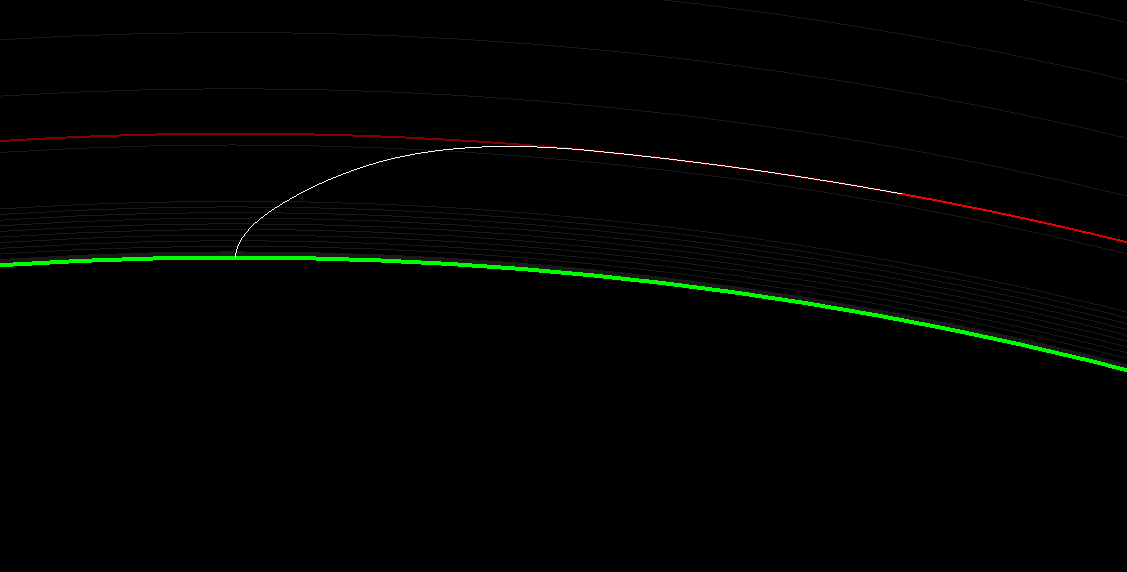
\includegraphics[width=\textwidth]{./220km.png}
  \caption{
    \label{fig:trajectory}
    Typical ascent to 220 km in a non-rotating Earth-centric reference frame. Trajectory shown in white. Final orbit shown in red.}
\end{figure}

It's clear from the trajectory in figure~\ref{fig:trajectory} that the trajectory starts out mostly vertical, where the atmosphere is densest. This prevents too much losses due to drag.

\subsection{Orbit insertion accuracy}
\begin{center}
  \begin{tabular}{ r | r  | l  l  }
     &   &  Achieved  \\
    Surface motion & Goal altitude & Perigee & Apogee \\
    \hline
    0 m/s & 170 km & 168.45 km & 169.52 km \\
    460 m/s & 170 km & 168.03 km & 170.26 km \\
    \hline
    0 m/s & 220 km & 218.49 km & 220.77 km \\
    460 m/s & 220 km  & 218.56 km & 219.21 km \\
    \hline
    0 m/s & 275 km & 274.41 km & 275.25 km \\
    460 m/s & 275 km & 275.30 km & 275.78 km
  \end{tabular}
\end{center}
It's clear that the algorithm works astonishingly well, with insertions just a few km in difference from the goal. It also works well for both equatorial and polar launch.

\subsection{Propellant consumption}
\begin{center}
  \begin{tabular}{ r | r  | l  l  }
     &   &   Propellant   \\
    Surface motion &  Goal altitude & Consumed & Remaining \\
    \hline
    0 m/s & 170 km & 512414 kg & 5986 kg \\
    460 m/s & 170 km & 509838 kg & 8562 kg \\
    \hline
    0 m/s & 220 km & 513645 kg & 4755 kg \\
    460 m/s & 220 km  & 511933 kg & 6467 kg \\
    \hline
    0 m/s & 275 km & 513562 kg & 4838 kg \\
    460 m/s & 275 km & 512208 kg & 6192 kg
  \end{tabular}
\end{center}
The propellant consumption was highest for the highest orbit goal, a reasonable expectation, but the difference between equatorial and polar launch was the lowest for the 220 km orbit goal.
This is further shown in the following table, comparing propellant usage for equatorial launch relative to polar launch:
\begin{center}
  \begin{tabular}{ r | l  l  }
     &   Propellant   \\
    Goal altitude & Consumed & Remaining \\
    \hline
    170 km & 99.40\% & 143 \% \\
    220 km & 99.67\% & 136 \% \\
    275 km & 99.74\% & 128 \%
  \end{tabular}
\end{center}



\section{Discussion}

By the results achieved, it's clear that orbital launch from the equator is better than launch from the poles. 
It is however interesting that the propellant consumption, for the orbit insertions simulated, is higher for polar launch to 220 km than it is for polar launch to 275 km.
This is likely an optimization problem, rather than related to the physics of the problem. A better error function might solve this,
but it could also be that the optimization function finds local minimums rather than a global minimum. 
A solution to this would be to sometimes run the algorithm for entirely random parameters, or increase the random scaling temporarily for every nth iteration. 

One must be careful just looking at the results however, as one might say that it is not by a huge margin that equatorial launch is better, 
but that's where the tyranny of the rocket equation comes into play.
This can be shown by introducing Tsiolkovsky's rocket equation
$$
\Delta v = v_{exhaust} \ln \frac{m_{final}}{m_{initial}}
$$
Solving for $m_{initial}$ gives
$$
\begin{aligned}
  m_{initial} = m_{final} \exp \left( -\frac{\Delta v}{v_{exhaust}} \right)
\end{aligned}
$$
If the goal is to accelerate 10000 kg of payload into a new velocity of 6 km/s with the second stage defined in the simulations, 
then reducing the fuel consumption by 2000 kg allows the usage of 10000 kg less fuel.
\begin{figure}[H]
  \begin{widepage}
    \centering
    \begin{minipage}{0.45\textwidth}
      \centering
      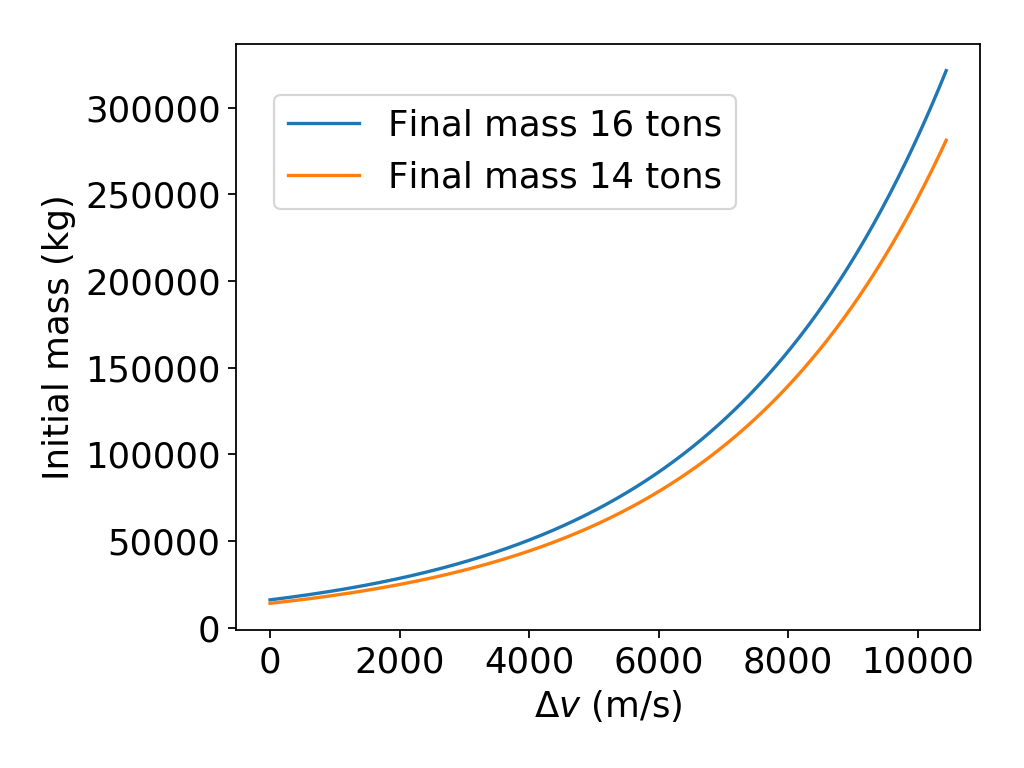
\includegraphics[width=\textwidth]{./plots/consumedToInitial.png}
      \caption{The initial mass necessary for the $v_{exhaust}$ used in simulation, for different final masses}
    \end{minipage}
    \hspace{0.025\textwidth}
    \begin{minipage}{0.45\textwidth}
      \centering
      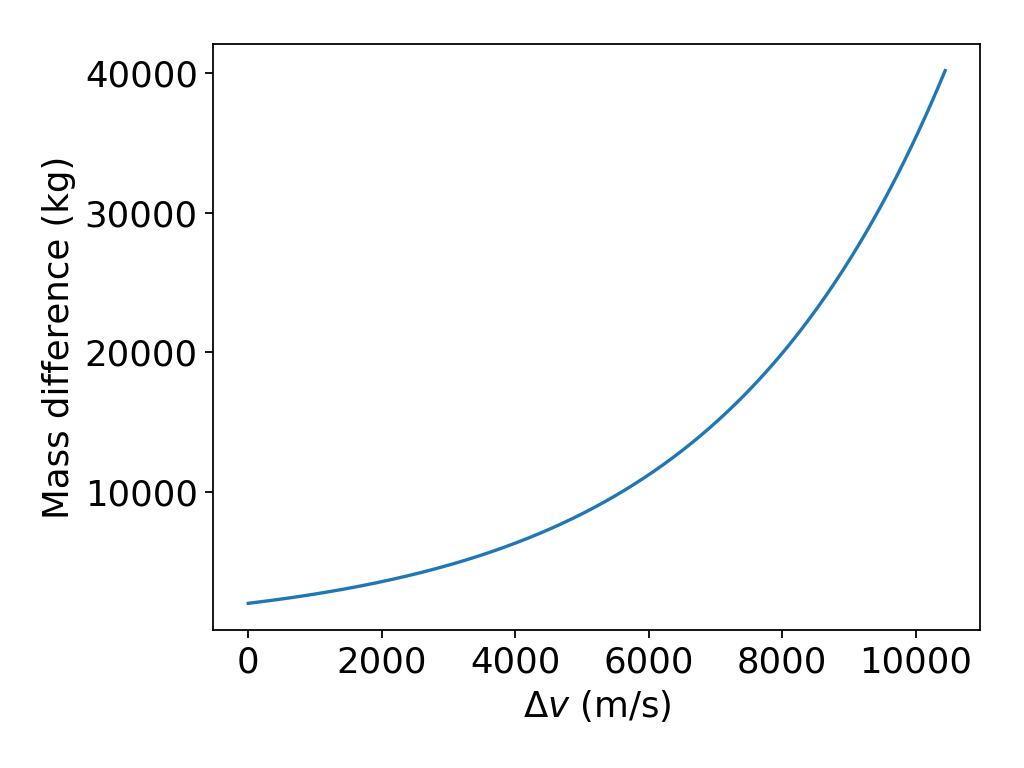
\includegraphics[width=\textwidth]{./plots/consumedToInitial_diff.png}
      \caption{The difference in initial mass for final masses of 14 and 16 tons}
    \end{minipage}
  \end{widepage}
\end{figure}

It was also interesting to see that the \textit{very} simple guidance algorithm was able to guide the rocket into an orbit very close to the goal.
It is definitely just scraping the surface of what is possible.
\begingroup
\raggedright
\bibliography{report}{}
\endgroup

\end{document}
